%%%%%%%%%%%%%%%%%%%%%%%%%%%%%
% Standard header for working papers
%
% WPHeader.tex
%
%%%%%%%%%%%%%%%%%%%%%%%%%%%%%

\documentclass[11pt]{article}

%%%%%%%%%%%%%%%%%%%%
%% Include general header where common packages are defined
%%%%%%%%%%%%%%%%%%%%

% general packages without options
\usepackage{amsmath,amssymb,bbm}




%%%%%%%%%%%%%%%%%%%%
%% Idem general commands
%%%%%%%%%%%%%%%%%%%%
%% Commands

\newcommand{\noun}[1]{\textsc{#1}}


%% Math

% Operators
\DeclareMathOperator{\Cov}{Cov}
\DeclareMathOperator{\Var}{Var}
\DeclareMathOperator{\E}{\mathbb{E}}
\DeclareMathOperator{\Proba}{\mathbb{P}}

\newcommand{\Covb}[2]{\ensuremath{\Cov\!\left[#1,#2\right]}}
\newcommand{\Eb}[1]{\ensuremath{\E\!\left[#1\right]}}
\newcommand{\Pb}[1]{\ensuremath{\Proba\!\left[#1\right]}}
\newcommand{\Varb}[1]{\ensuremath{\Var\!\left[#1\right]}}

% norm
\newcommand{\norm}[1]{\| #1 \|}


% amsthm environments
\newtheorem{definition}{Definition}



%% graphics

% renew graphics command for relative path providment only ?
%\renewcommand{\includegraphics[]{}}








% geometry
\usepackage[margin=2cm]{geometry}

% layout : use fancyhdr package
\usepackage{fancyhdr}
\pagestyle{fancy}

\makeatletter

\renewcommand{\headrulewidth}{0.4pt}
\renewcommand{\footrulewidth}{0.4pt}
%\fancyhead[RO,RE]{\textit{Working Paper}}
\fancyhead[RO,RE]{\textit{ECTQG 2015}}
%\fancyhead[LO,LE]{G{\'e}ographie-Cit{\'e}s/LVMT}
\fancyhead[LO,LE]{An Algorithmic Systematic Review}
\fancyfoot[RO,RE] {\thepage}
\fancyfoot[LO,LE] {\noun{J. Raimbault}}
\fancyfoot[CO,CE] {}

\makeatother


%%%%%%%%%%%%%%%%%%%%%
%% Begin doc
%%%%%%%%%%%%%%%%%%%%%

\begin{document}








\title{LUTECIA : a toy-model to study the role of governance in multi-scale metropolitan transportation/land-use interactions\bigskip\\
\textit{Working Paper}
}
\author{\noun{Juste Raimbault}, \noun{Florent Le Nechet}}
\date{September 2015}




\maketitle

\justify


\begin{abstract}

\end{abstract}


%%%%%%%%%%%%%%%%%%%%%%
%% Sec 1 : Introduction
%%%%%%%%%%%%%%%%%%%%%%
\section{Introduction}

% thematic context, purpose, etc

%%%%%%%%%%%%%%%%%%%%%%
\subsection{Context}



%%%%%%%%%%%%%%%%%%%%%%
\subsection{Research question}






%%%%%%%%%%%%%%%%%%%%%%
\subsection{Proposed approach}


Model structure : scheme and modules :

\begin{itemize}
\item LU stands for Land Use module
\item T stands for Transport module
\item EC stands for Evaluation of Cooperation module
\item I stands for Infrastructure provision module
\item A stands for Agglomeration economies module
\end{itemize}


Details on multiple time scales ; corresponding stochasticity level of the model.






%%%%%%%%%%%%%%%%%%%%%%
%% Sec 2 : Model description
%%%%%%%%%%%%%%%%%%%%%%
\section{Model description}



%%%%%%%%%%%%%%%%%%%%%%
\subsection{Global architecture}



%%%%%%%%%%%%%%%%%%%%%%
\subsection{Modules description}


\subsubsection{Settings}



\subsubsection{Land-Use evolution}




Land-Use module : we assume that residential/employments relocations are at equilibrium at the time scale of a tick, that corresponds to transportation infrastructure evolution time scale which is much larger (Bretagnolle, 2009).

We take a Cobb-douglas function for utilities of actives/employments at a given cell
\[
U_i (A) = X_i(A)^{\gamma_A}\cdot {F_i(A)}^{1-\gamma_A} ; F_i(A) = \frac{1}{A_i E_i}
\]
\[
U_j (E) = X_j(E)^{\gamma_E}\cdot {F_j(E)}^{1-\gamma_E} ; F_j(E) = 1
\]

where $X_i(A) = A_i\cdot \sum_j{E_j \exp{\left(-\lambda\cdot d_{ij}\right)}}$ and $X_j(E) = E_j\cdot \sum_i{A_i \exp{\left(-\lambda\cdot d_{ij}\right)}}$.

Relocations are then done deterministically following a discrete choice model :
\[
A_i(t+1) = \sum_i{A_i(t)}\cdot\frac{\exp{(\beta U_i(A))}}{\sum_i{\exp{(\beta U_i(A))}}}
\]
\[
E_j(t+1) = \sum_j{E_j(t)}\cdot\frac{\exp{(\beta U_j(E))}}{\sum_j{\exp{(\beta U_j(E))}}}
\]





\subsubsection{Transportation}



Transportation module : computation of flows $\phi_{ij}$ by solving on $p_i,q_j$ by a fixed point method (Furness algorithm), the system of gravital flows
\[
\begin{cases}
\phi_{ij} = p_i q_j A_i E_j \exp{\left(-\lambda_{tr} d_{ij}\right)}\\
\sum_k \phi_{kj} = E_j ; \sum_k \phi_{ik} = A_i\\
p_i = \frac{1}{\sum_k{q_k E_k \exp{(-\lambda_{tr}d_{ik})}}} ; q_j = \frac{1}{\sum_k{p_k A_k \exp{(-\lambda_{tr}d_{kj})}}} 
\end{cases}
\]

Trajectories then attributed by effective shortest path, and corresponding congestion $c$ obtained (no Wardrop equilibrium). 

Speed of network given by BPR function $v(c) = v_0 \left(1 - \frac{c}{\kappa}\right)^{\gamma_c}$. Congestion not used in current studies (infinite capacity $\kappa$).





\subsubsection{Governance}

% from previous wp on governance module only.



The workflow for transportation network development is the following :

\begin{itemize}

\item At each time step, $N$ new road segments are built. Choice between local and global is still done through uniform drawing with probability $\xi$. In the case of local building, roads are attributed successively to mayors with probabilities $\xi_i$, what means that richer areas may get many roads. It stays consistent with the thematic assumption than each road correspond to the allocation of one public market which are done independantly (with $N$ becoming greater, this assumption should be relaxed as attribution of subventions to local areas is of course not proportional to wealth, but we assume that it stays true with small $N$ values). 

\item Areas building a road without neighbors doing it follow the standard procedure to develop the road network.

\item Neighbor areas building a road will enter negociations. We assume in this first simple version of the model that ony bilateral negociations may occur. Therefore, in the case of clusters with more than two areas, pairing is done at random (uniform drawing) between neighbors until all areas are paired.

\item Possible strategies for players (negociating areas, $i=1,2$) are : staying alone ($A$) and collaborating ($C$). Strategies are chosen simultaneously (non-cooperative game) as detailed after. For $(C,A)$ and $(A,C)$ couples, the collaborating agent loose its investment and cannot build a road whereas the other continues his buiseness alone. For $(A,A)$ both act as alone, and for $(C,C)$ a common development is done. We denote $Z^{\ast}_i(S_1,S_2)$ the optimal infrastructure for area $i$ with $(S_1,S_2)\in \{(A,C),(C,A),(A,A)\}$ which are determined the standard way in each zone separately, and $Z^{\ast}_C$ the optimal common infrastructure computed with a 2 segments infrastructure on the union of both areas, which corresponds to the case where both strategies are $C$. Marginal accessibilities for area $i$ and infrastucture $Z$ is defined as $\Delta X_i(Z)=X^Z_i - X_i$. We introduce the costs of construction which are necessary to build the payoff matrix. They are assumed spatially uniform and noted $I$ for a road segment, whereas a 2 road segment will cost $2\cdot I - \delta I$ ($\delta I > 0$ cost gain of common technical means, assumed to be equally shared). An interesting generalisation would be to divise costs proportionnaly to wealth in the case of a collaboration. The payoff matrix of the game is the following, with $\kappa$ a normalization constant (``price of acessibility'') :

\medskip
\hfill
\begin{tabular}{ |c|c|c| } 

 \hline
 1 $|$ 2  & C & A \\ \hline
 C & $U_i = \kappa \cdot \Delta X_i(Z^{\ast}_C) - I + \frac{\delta I}{2}$
   & $\begin{cases}U_1 = -I + \frac{\delta I}{2} \\U_2 = \kappa \cdot \Delta X_2(Z^{\ast}_2)-I + \frac{\delta I}{2}\end{cases}$ \\ \hline
 A & $\begin{cases}U_1 = \kappa \cdot \Delta X_1(Z^{\ast}_1)-I + \frac{\delta I}{2}\\U_2 = -I + \frac{\delta I}{2}\end{cases}$
   & $U_i = \kappa \cdot \Delta X_i(Z^{\ast}_i) - I$ \\
 \hline
\end{tabular}
\hfill\hfill
\medskip

We have a typical coordination game for which it is clear that no strategy is dominant for any player. In a probabilistic mixed-strategy case, there always exists a Nash equilibrium that we can easily determine in our case. It is reasonable to make such an assumption since negociations take generally some time during which agents are able to find the way to optimize rationaly their expected utility. If $\Pb{S_1=C} = p_1$ and $\Pb{S_2=C} = p_2$, we have

\[
\begin{split}
\Eb{U_1} & =p_1 p_2 U_1(C,C) + p_1\cdot (1-p_2) U_1(C,A) + p_2 \cdot (1-p_1) U_1(A,C) + (1-p_1)(1-p_2) U_1(A,A)\\
& = p_1 \cdot \left[ p_2 \cdot \left(\kappa \cdot \Delta X_1(Z^{\ast}_C) - \frac{\delta I}{2} \right) - \kappa \cdot \Delta X_1(Z^{\ast}_1) + I\right] + p_2\cdot\frac{\delta I}{2} + \kappa\cdot\Delta X_1(Z^{\ast}_1)-I
\end{split}
\]

Optimizing the expected utility along $p_1$ (the variable on which agent 1 has control) imposes the condition on $p_2$

\[
\frac{\partial \Eb{U_1}}{\partial p_1} = 0 \iff p_2 = \frac{\Delta X_1(Z^{\ast}_1)-\frac{I}{\kappa}}{\Delta X_1(Z^{\ast}_C) - \frac{\delta I}{2\cdot \kappa}}
\]

We obtain the same way

\[
p_1 = \frac{\Delta X_2(Z^{\ast}_2)-\frac{I}{\kappa}}{\Delta X_2(Z^{\ast}_C) - \frac{\delta I}{2\cdot\kappa}}
\]

Note that we can directly interpret these expressions, as a player chances to cooperate will decrease with the potential gain of the other player, what is intuitive for a competitive game. It also forces feasibility conditions on $I$ and $\delta I$ to keep a probability, that are $I \leq \kappa\cdot \min(\Delta X_1(Z^{\ast}_1),\Delta X_2(Z^{\ast}_2))$ (binary positive cost-benefit conditions) and $I-\delta I > \kappa \cdot \max_i (\Delta X_i(Z^{\ast}_i)-\Delta X_i(Z^{\ast}_C))$. As soon as accessibility difference stay relatively small, both shall be compatible when $\delta I \ll I$, giving corresponding boundaries for $I$.

\item Agents make choice of strategy following uniform drawings with probability computed above. Corresponding infrastructures are built, and in the case of choices $(C,C)$, towns merge in a single one with new corresponding variables (employment, actives, etc. ).


\end{itemize}











TODO : check models with $n$ agents ?

Mixed nash equilibrium formula : 

\[
p_i = \frac{J}{\Delta X_{\bar{i}}{Z^{\star}_{C}} - \Delta X_{\bar{i}}{Z^{\star}_{\bar{i}}}}
\]


Discrete choices model :

\[
U_i(C) - U_i(NC) = p_{\bar{i}} \left( \Delta X_{i}{Z^{\star}_{C}} - \Delta X_{i}{Z^{\star}_{i}}\right) - J
\]

\[
p_i = \frac{1}{1 + \exp{\left(-\beta_{DC}\cdot \left(\frac{\Delta X_{i}{Z^{\star}_{C}} - \Delta X_{i}{Z^{\star}_{i}}}{1 + \exp{\left(- \beta_{DC}(p_i \cdot (\Delta X_{\bar{i}}{Z^{\star}_{C}} - \Delta X_{\bar{i}}{Z^{\star}_{\bar{i}}}) - J)\right)}} - J \right)\right)}}
\]





%%%%%%%%%%%%%%%%%%%%%%
%% Sec 2 : Implementation
%%%%%%%%%%%%%%%%%%%%%%
\section{Implementation}



\subsection{Implementation choices}

Effective distances computation

\begin{itemize}
\item Euclidian distance matrix $d(i,j)$ computed analytically
\item Network shortest paths between network intersections (rasterized network) updated in a dynamic way (addition of new paths and update/change of old paths if needed when a link is added), correspondance between network patches and closest intersection also updated dynamically ; $O(N_{inters}^3)$
\item Weak component clusters and distance between clusters updated ; $O(N_{nw}^2)$
\item Network distances between network patches updated, through the heuristic of only minimal connexions between clusters ; $O(N_{nw}^2)$
\item Effective distances (taking paces/congestion into account) updated as minimum between euclidian time and $\min_{C,C'}{d(i,C)+d_{nw}(p_C(i),p_C'(j))+d(C',j)}$ ; $O(N_{clusters}^2\cdot N^2)$ [Approximed with $\min_C$ only in the implementation, consistent within the interaction ranges $\sim$ 5 patches taken in the model]. 
\end{itemize}





The model was implemented in \texttt{NetLogo}~\cite{wilensky1999netlogo} because of its exploratory and interactive nature. A particular care was taken for the computation of accessibilities and shortest paths, as a dynamic reevaluation of network distance is necessary for each new potential infrastructure, what become rapidly a computational burden. We use thus a dynamical programming shortest path computation, inspired from~\cite{tretyakov2011fast}, using distance matrices updates instead of shortest paths full computation at each step. See details in architectural precisions in Appendix~\ref{app:bibliography}


%%%%%%%%%%
\begin{figure}
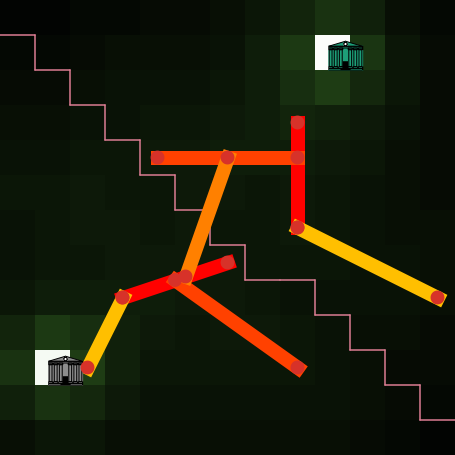
\includegraphics[width=0.5\textwidth]{figures/ex_collab_0}
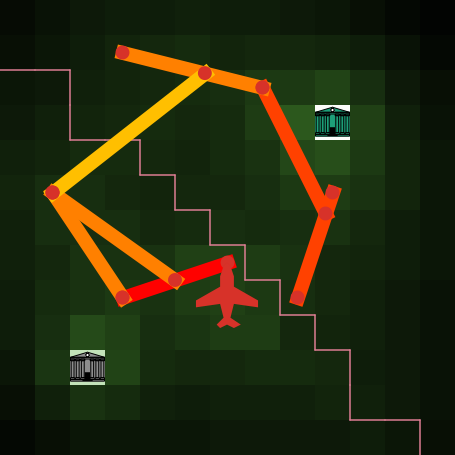
\includegraphics[width=0.5\textwidth]{figures/ex_dc_finalCollab}\\
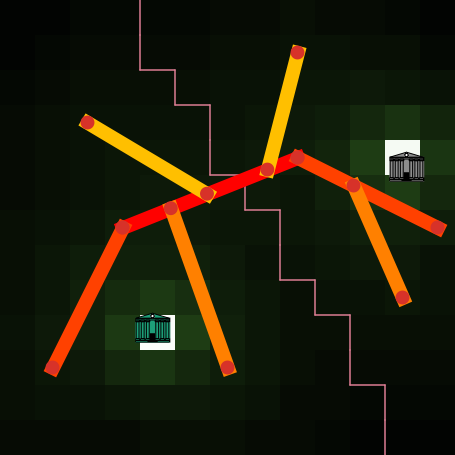
\includegraphics[width=0.5\textwidth]{figures/ex_simpleNash_0}
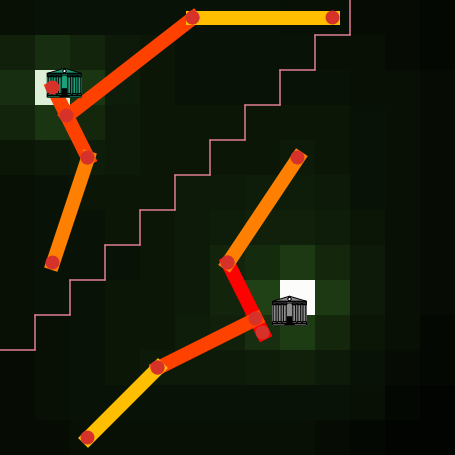
\includegraphics[width=0.5\textwidth]{figures/example_nocollab_0}
\caption[Examples of final configurations]{Examples of final configurations, with or without externality, for different values of cooperation parameters.}
\label{fig:luteciaexample}
\end{figure}
%%%%%%%%%%


%%%%%%%%%%
\begin{figure}
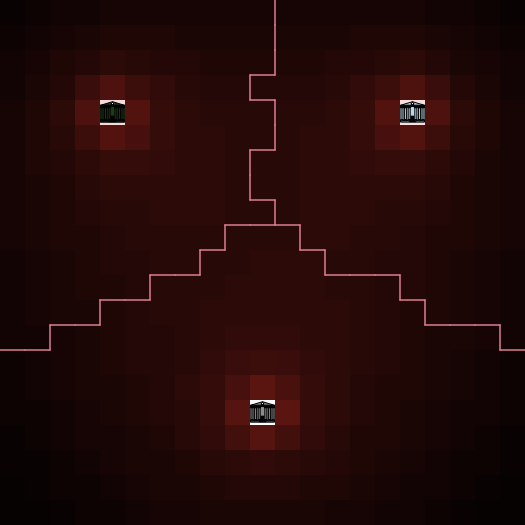
\includegraphics[width=0.5\textwidth]{figures/_MEAN_ACC}
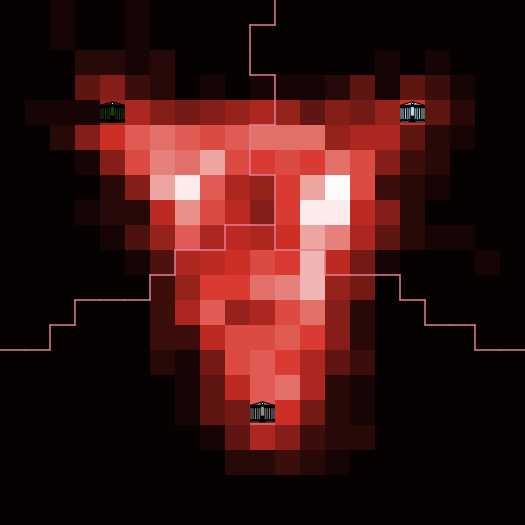
\includegraphics[width=0.5\textwidth]{figures/_NW_FREQ}
\caption[Validation of network exploration heuristic]{Validation of network exploration heuristic : mean accessibility(left) and network positions on 500 realizations on the same initial configuration. The optimal distribution of network validates network generation heuristic.}
\label{fig:luteciavalid}
\end{figure}
%%%%%%%%%%%








%%%%%%%%%%%%%%%%%%%%%%
%% Sec 2 : Validation
%%%%%%%%%%%%%%%%%%%%%%
\section{Experiments and validation}


We show in Fig.~\ref{fig:luteciaexample} and Fig.\ref{fig:luteciavalid} examples of obtained configurations and preliminary validation of governance and network growth heuristic. Internal validation and external validation through stylized facts, and model explorations, including statistical analysis of model behavior, are provisory for now and not presented here (see~\cite{le2015modeling} for preliminary results).







%%%%%%%%%%%%%%%%%%%%%%
\subsection{Validation of the LU-T joint modules}

List of key processes implemented, and associated parameters (\textit{ref tableau qui indique l'ensemble des paramètres du modèle}):
\begin{itemize}
\item Production of flows, parameters ?
\item Relocation of inhabitants, parameters ?
\item Relocation of activities, parameters ?
\end{itemize}


Stylized facts to retrieve : 
\begin{itemize}
	\item Stability of monocentric structure with one CBD cell and descending density gradient
	\item Response to a new spider network (forced) : sprawl that keep the mathematical form of the descending density gradient
	\item Response to a change in cost of energy (parameter $\lambda$) : sprawl of inhabitants bigger than the sprawl of jobs
\end{itemize}





%%%%%%%%%%%%%%%%%%
\subsection{Validation of the LU-T-I joint modules}

List of key processes implemented, and associated parameters (\textit{ref tableau qui indique l'ensemble des paramètres du modèle}):
\begin{itemize}
\item Creation of a new infrastructure to maximize new accessibility of a given stakeholder
\end{itemize}

Stylized facts to retrieve :
\begin{itemize}
	\item Reasonable path dependancy : form follow network, but not too rapidly
	\item Optimal routes correspond to physical least effort law which network better link the four points of a square $\rightarrow$ not a cross, but a \texttt{>-<} shape
\end{itemize}





%%%%%%%%%%%%%%%%%%%%%%
\subsection{Validation of the LU-T-I-A joint modules}


List of key processes implemented, and associated parameters (\textit{ref tableau qui indique l'ensemble des paramètres du modèle}):
\begin{itemize}
\item Creation of new jobs in the region to account for the increase of overall accessibility
\item Spread of this jobs in a few places with exceptional amenities
\item Adaptation of number of inhabitants and relocation
\end{itemize}


Stylized facts to retrieve : 
\begin{itemize}
	\item Increase of accessibility of a monocentric region shall fall within reasonable interval (see litterature such as Desjardin in Paris region) 
	\item Resulting increase of number of jobs shall fall within reasonable interval (see litterature on agglomeration economies)
\end{itemize}





%%%%%%%%%%%%%%%%%%%%%%
\subsection{Validation of the LU-T-EC-I-A joint modules}

List of key processes implemented, and associated parameters (\textit{ref tableau qui indique l'ensemble des paramètres du modèle}):
\begin{itemize}
	\item Choice between local stakeholders developments of integrated regional development
	
\end{itemize}


Stylized facts to retrieve : 
\begin{itemize}
	\item For a region with obvious no need to collaborate (e.g. cities far away from each other) : collaboration never occurs
	\item For a region with obvious need to collaborate (e.g. large elasticity of jobs regarding to overall accessibility and urban form such as better link for local purpose and regional purpose are self-evident \textbf{and} different
	\item For a intermediate region, the relative share of cooperation / non-cooperation outcome is quite stable among replications of the simulation
\end{itemize}



%%%%%%%%%%%%%%%%%%%%%%
%% Sec 5 : Exploration
%%%%%%%%%%%%%%%%%%%%%%
\section{Model exploration}

%Quand on en sera là ce sera super, mais pour mémoire, je trouve qu'on a pas assez travaillé l'aspect forme urbaine initiale.












%%%%%%%%%%%%%%%%%%%%%%
%% Sec 6 : Discussion
%%%%%%%%%%%%%%%%%%%%%%
\section{Discussion}







%%%%%%%%%%%%%%%%%%%%%%
%% Conclusion
%%%%%%%%%%%%%%%%%%%%%%
\section*{Conclusion}





%%%%%%%%%%%%%%%%%%%%
%% Biblio
%%%%%%%%%%%%%%%%%%%%

\bibliographystyle{apalike}
\bibliography{}


\end{document}




